\newpage
%
\subsection{Списание материалов}
\label{bp:MatOutput}

\subsubsection{Списание бумаги и картона}


Бригадир ГА получает плановое задание на гофроагрегат (рис. \ref{pic:f8b} - \ref{pic:f8a}),
определяет потребность в сырье, в устной форме передает ее кладовщику. Кладовщик с водителем погрузчика находят необходимое сырье и подают на гофроагрегат.

Сырьевые остатки в виде частично использованных рулонов обратно на склад не возвращаются. Учет частично использованных рулонов ведется производством в штуках, а не в килограммах (отсутствуют весы).

Все переданное на производство сырье кладовщик вносит в таблицу MS EXCEL с указанием даты передачи.

Кладовщик ведет ведомость списания сырья, которую подписывает бригадир, и передает ее в бухгалтерию (рис. \ref{pic:f26}).

Все остатки формируются ежедневно в таблице MS EXCEL (рис. \ref{pic:f2}).

На складе сырья планируется выполнить разметку для ячеечного хранения продукции (рис. \ref{pic:f4}). 




\subsection{Учет вспомогательных материалов}

Каждый день кладовщик сверяет остатки ТМЦ на складе с данными таблицы MS EXCEL (рис. \ref{pic:f2}) и вносит необходимые корректировки.

Деревянные поддоны учитываются отдельно и выдаются на производство по ведомости  (рис. \ref{pic:f27}).





\begin{figure}
\begin{center}
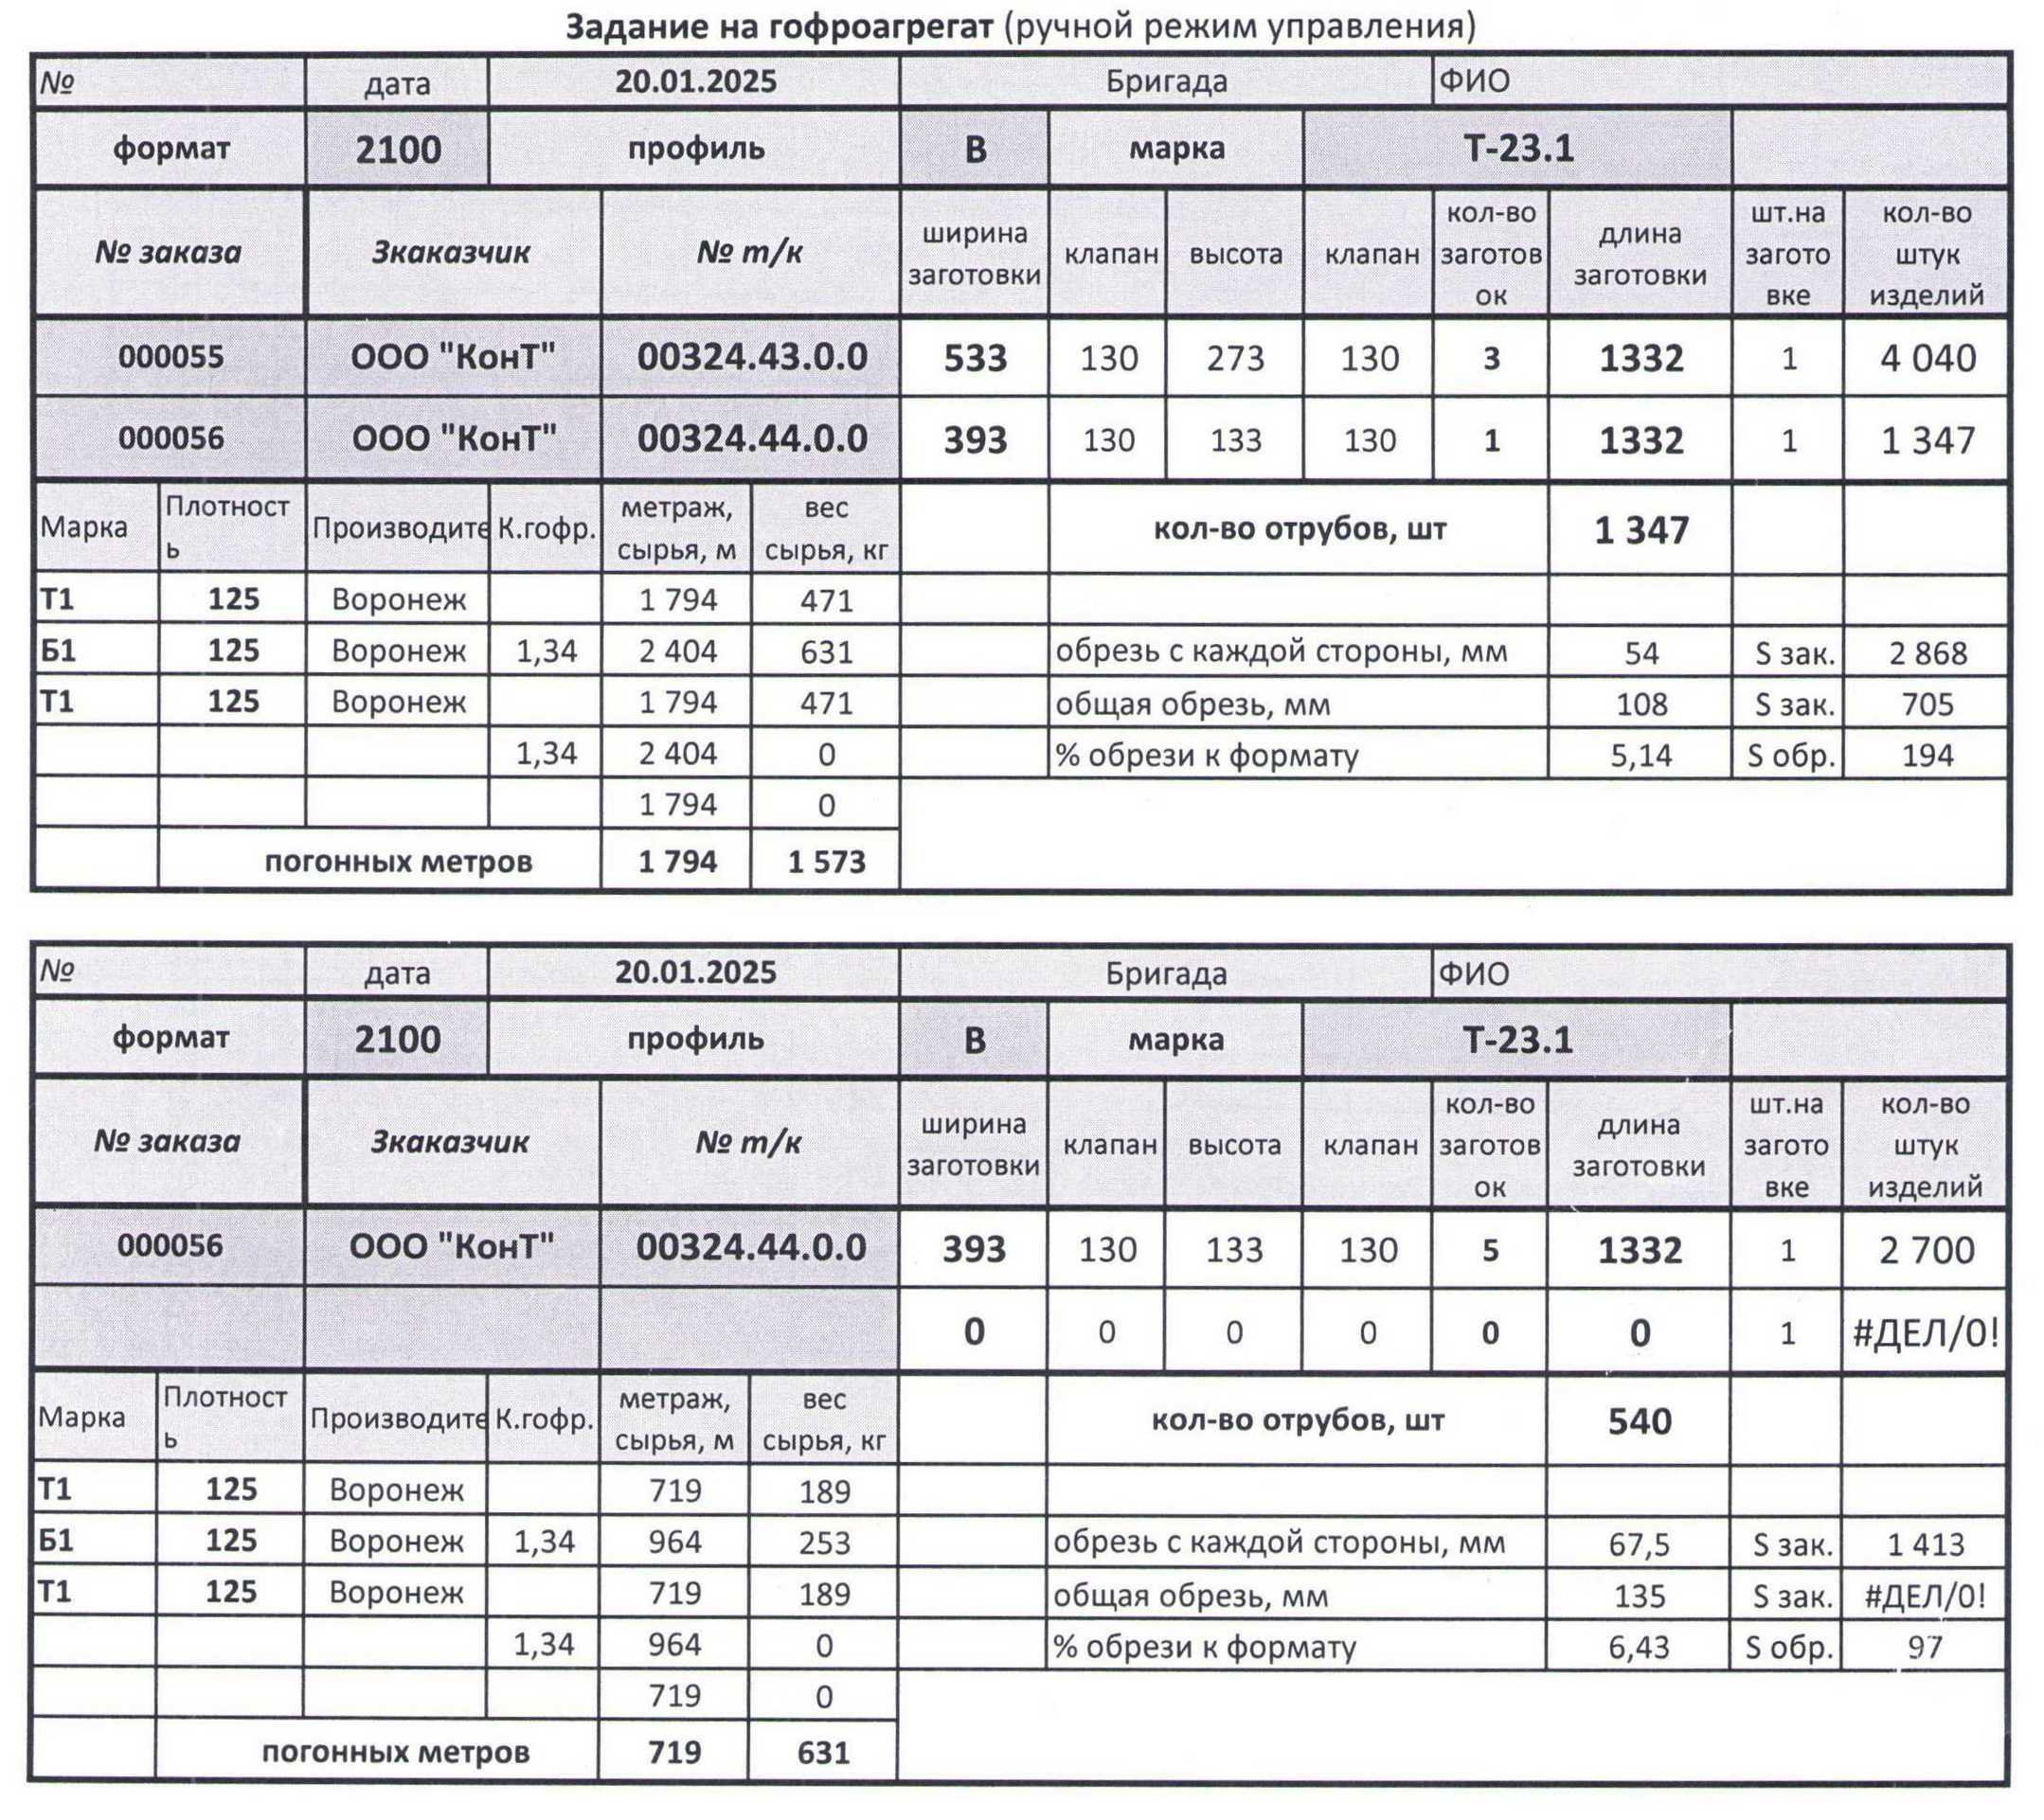
\includegraphics[height=0.94\textheight, width=\textwidth, keepaspectratio]{Pics/f8b.jpg}
\end{center}
\caption{Задание на ГА. Часть 1}
\label{pic:f8b}
\end{figure}

\begin{figure}
\begin{center}
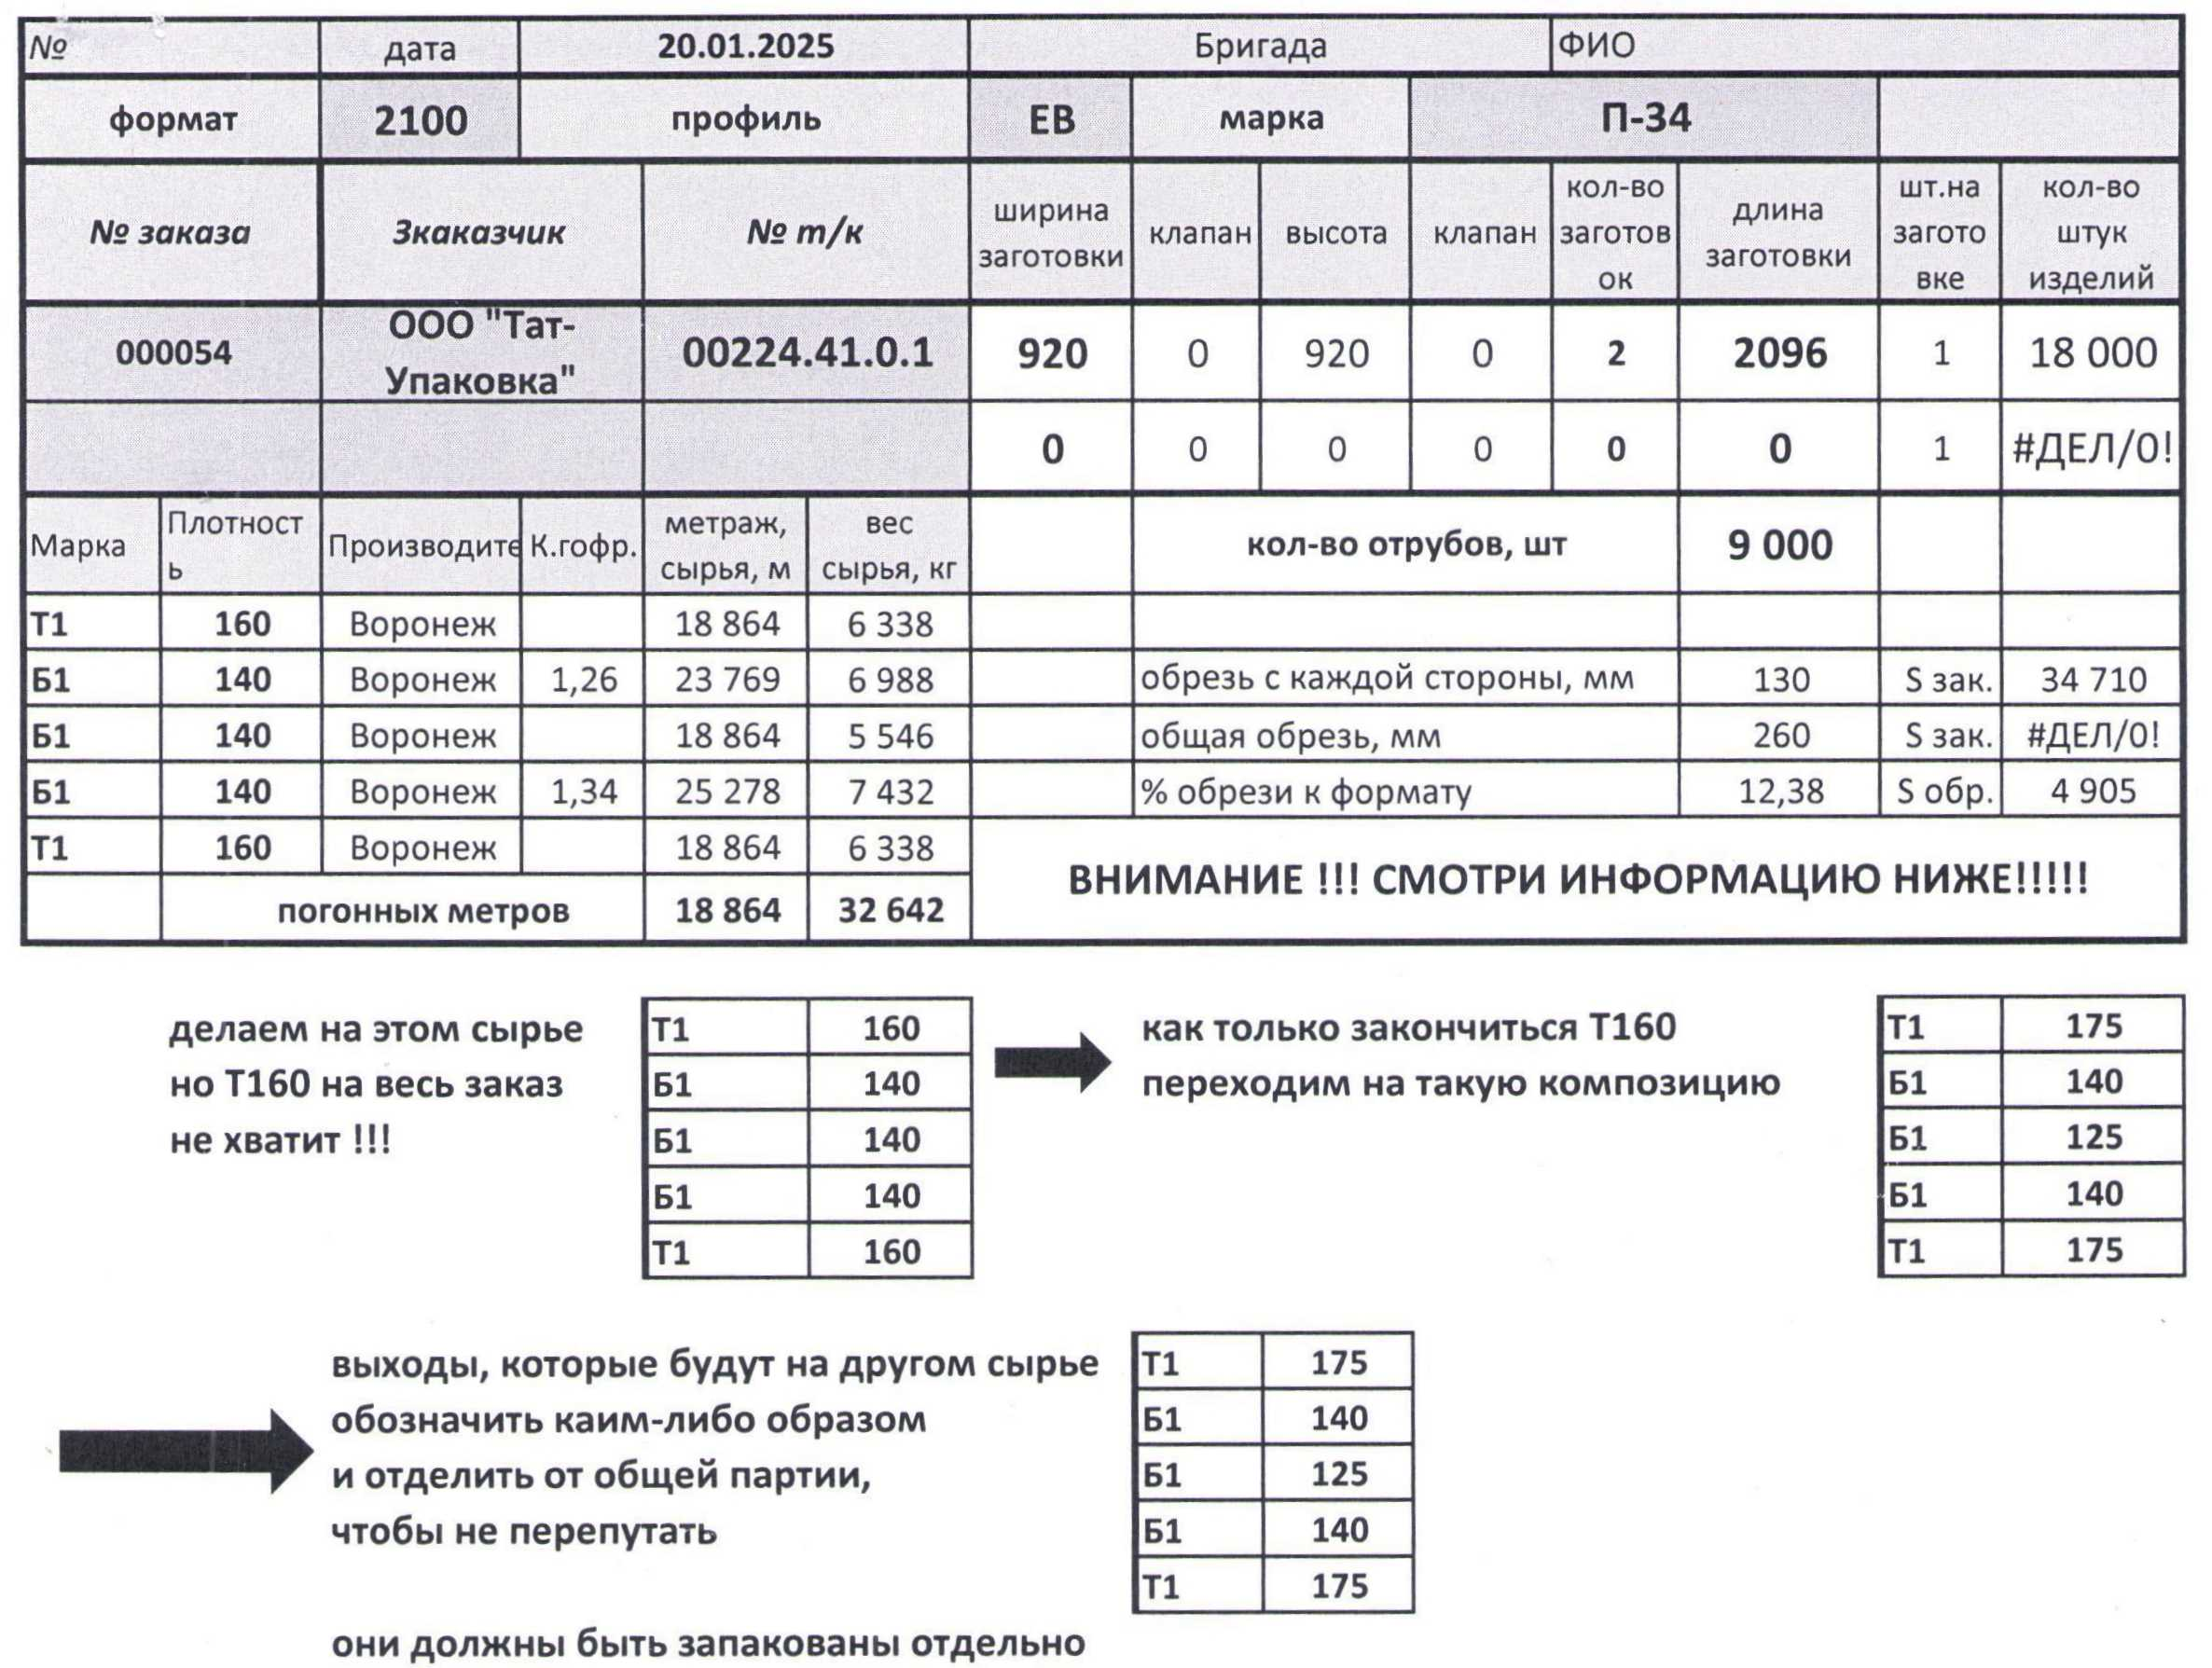
\includegraphics[height=0.94\textheight, width=\textwidth, keepaspectratio]{Pics/f8a.jpg}
\end{center}
\caption{Задание на ГА. Часть 2}
\label{pic:f8a}
\end{figure}

\begin{figure}
\begin{center}
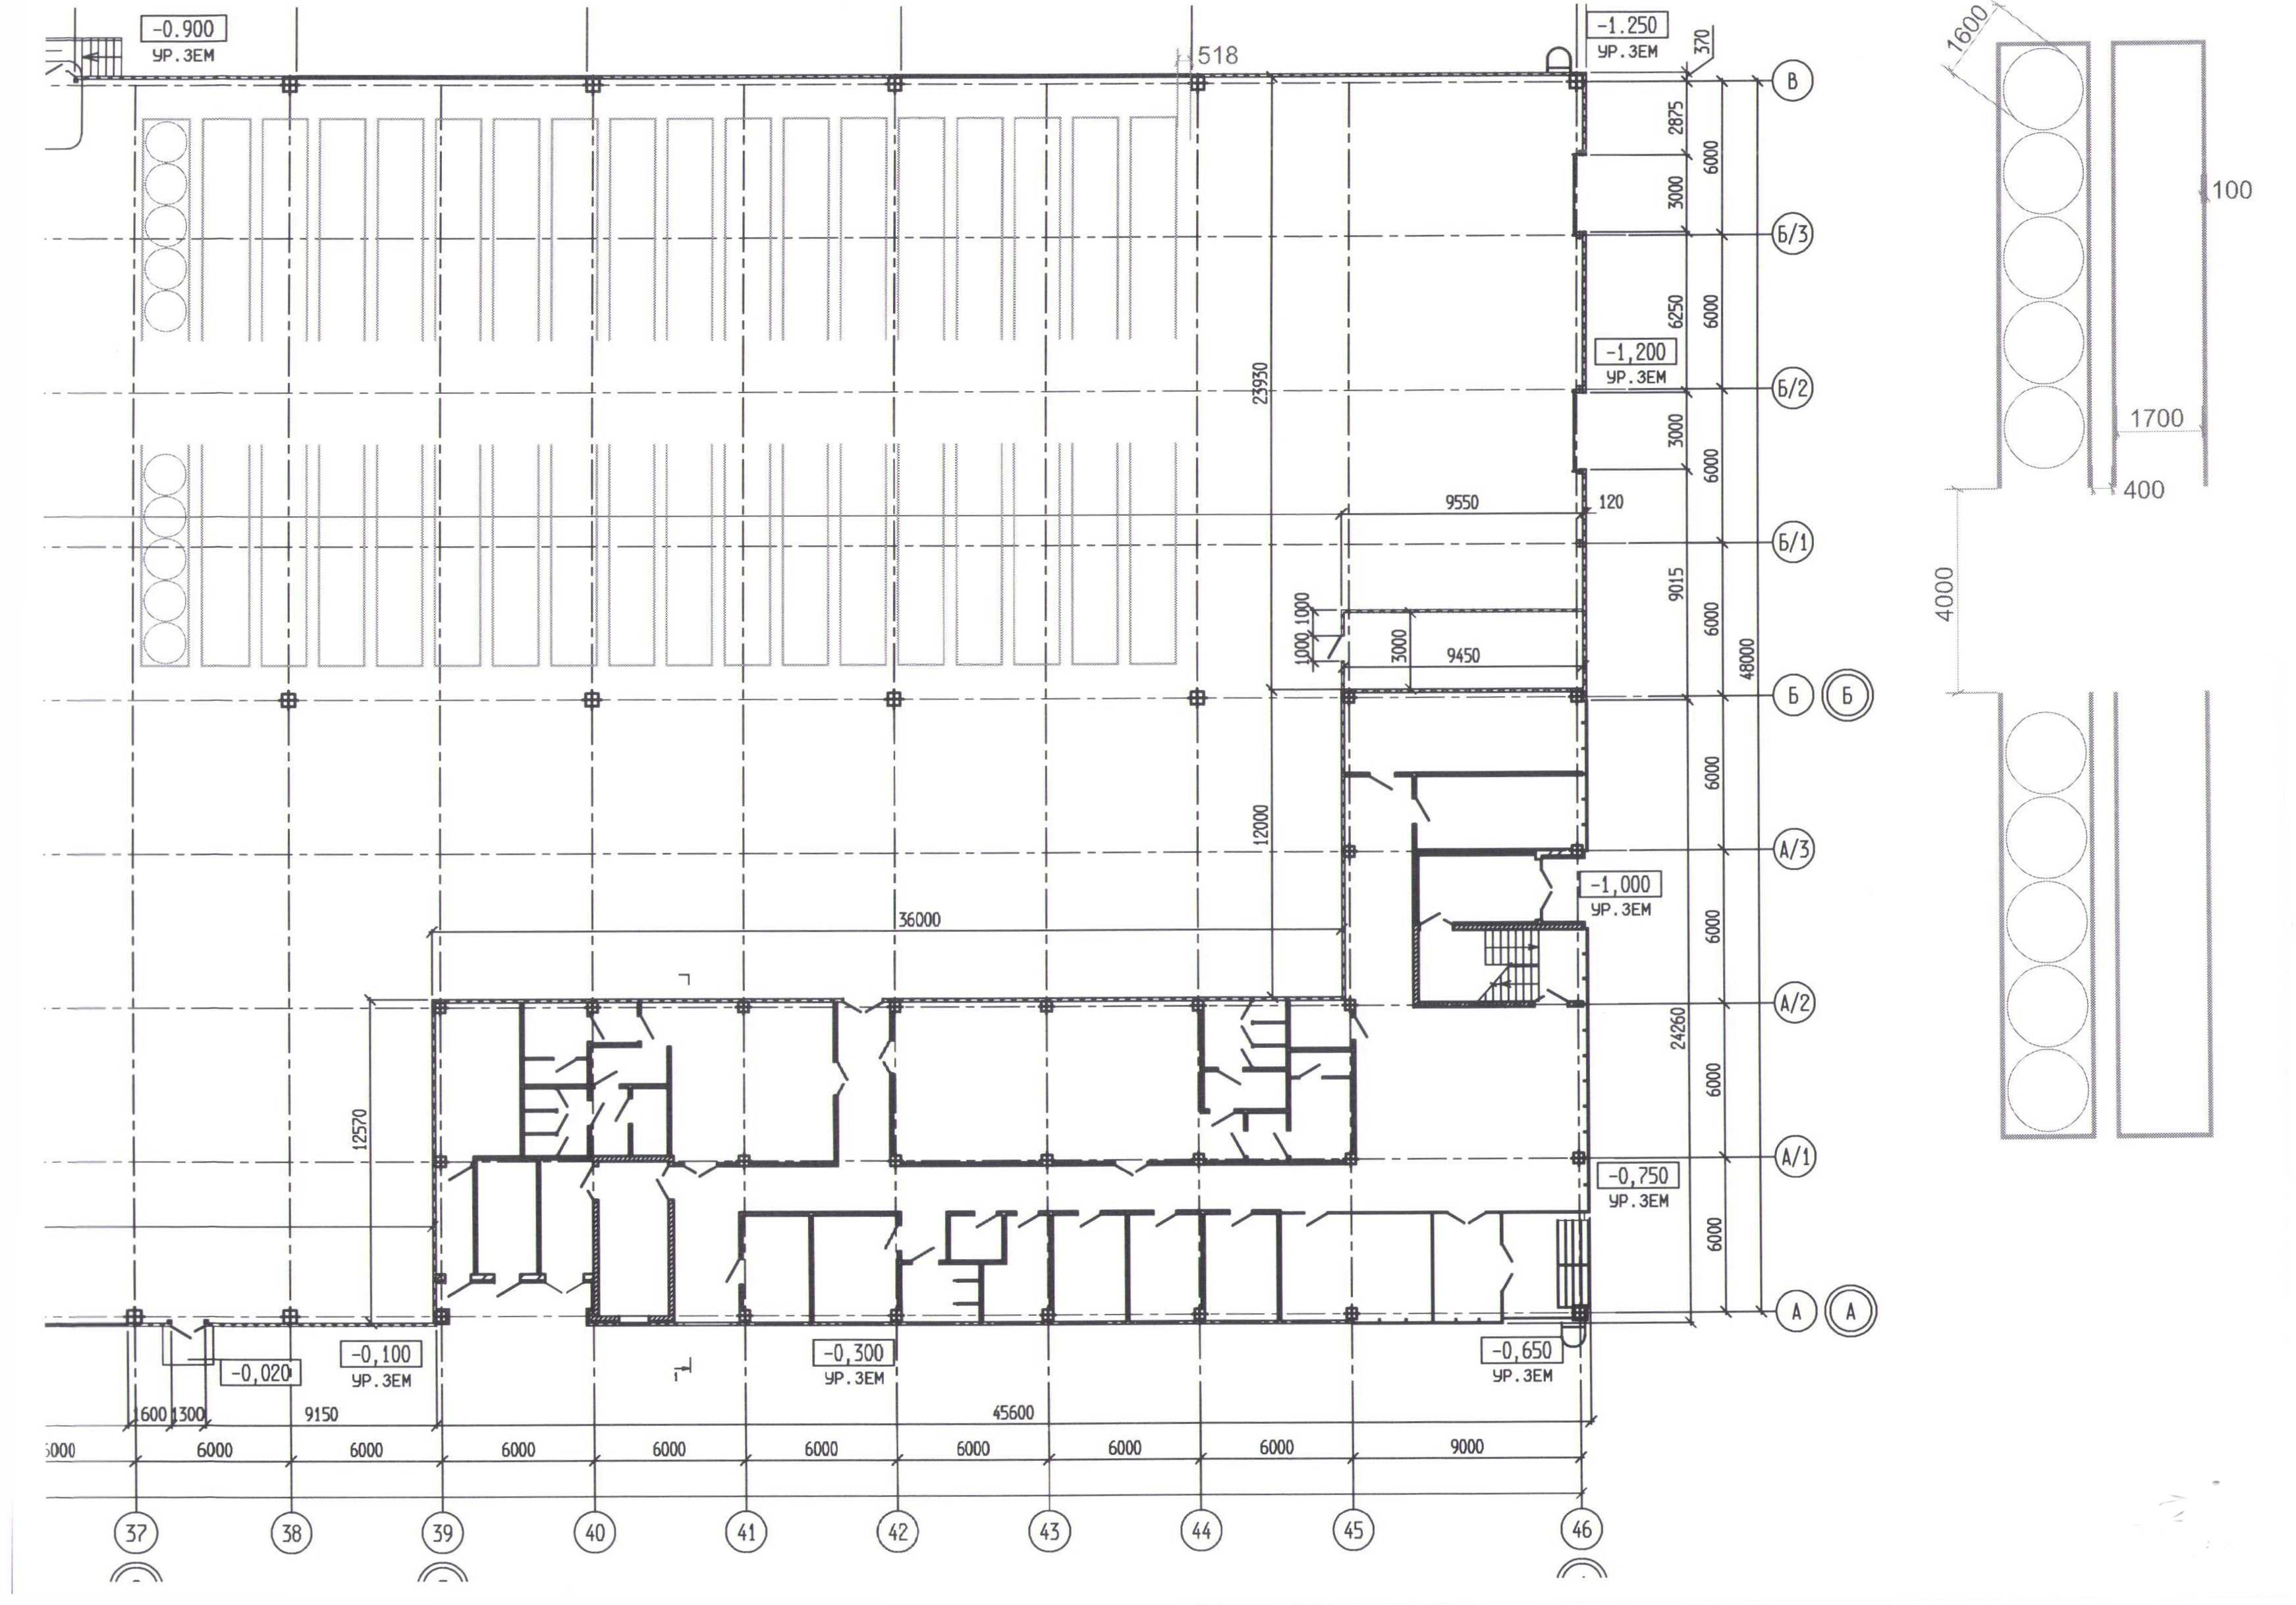
\includegraphics[height=0.94\textheight, width=\textwidth, angle=90, keepaspectratio]{Pics/f4.jpg}
\end{center}
\caption{Склад сырья. Разметка предусматривающая ячеистое хранение продукции}
\label{pic:f4}
\end{figure}

\begin{figure}
\begin{center}
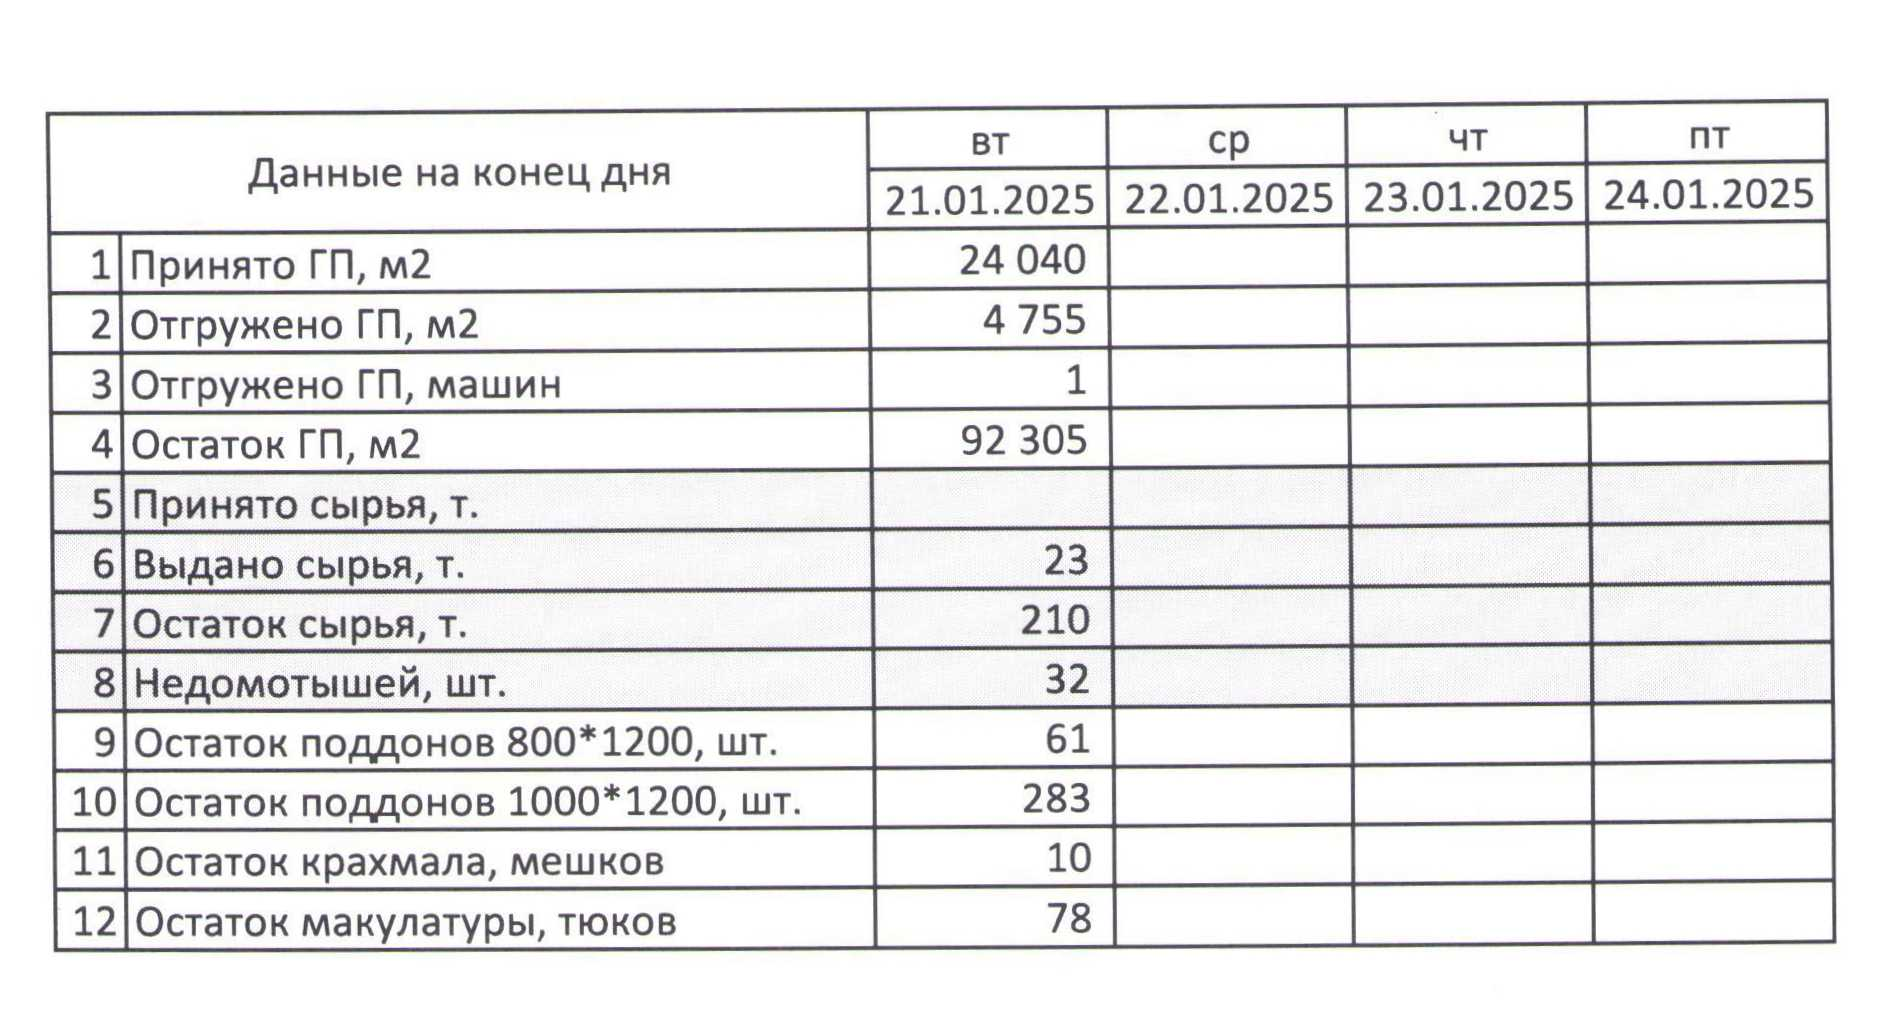
\includegraphics[height=0.94\textheight, width=\textwidth, keepaspectratio]{Pics/f2.jpg}
\end{center}
\caption{Остатки ТМЦ}
\label{pic:f2}
\end{figure}

\begin{figure}
\begin{center}
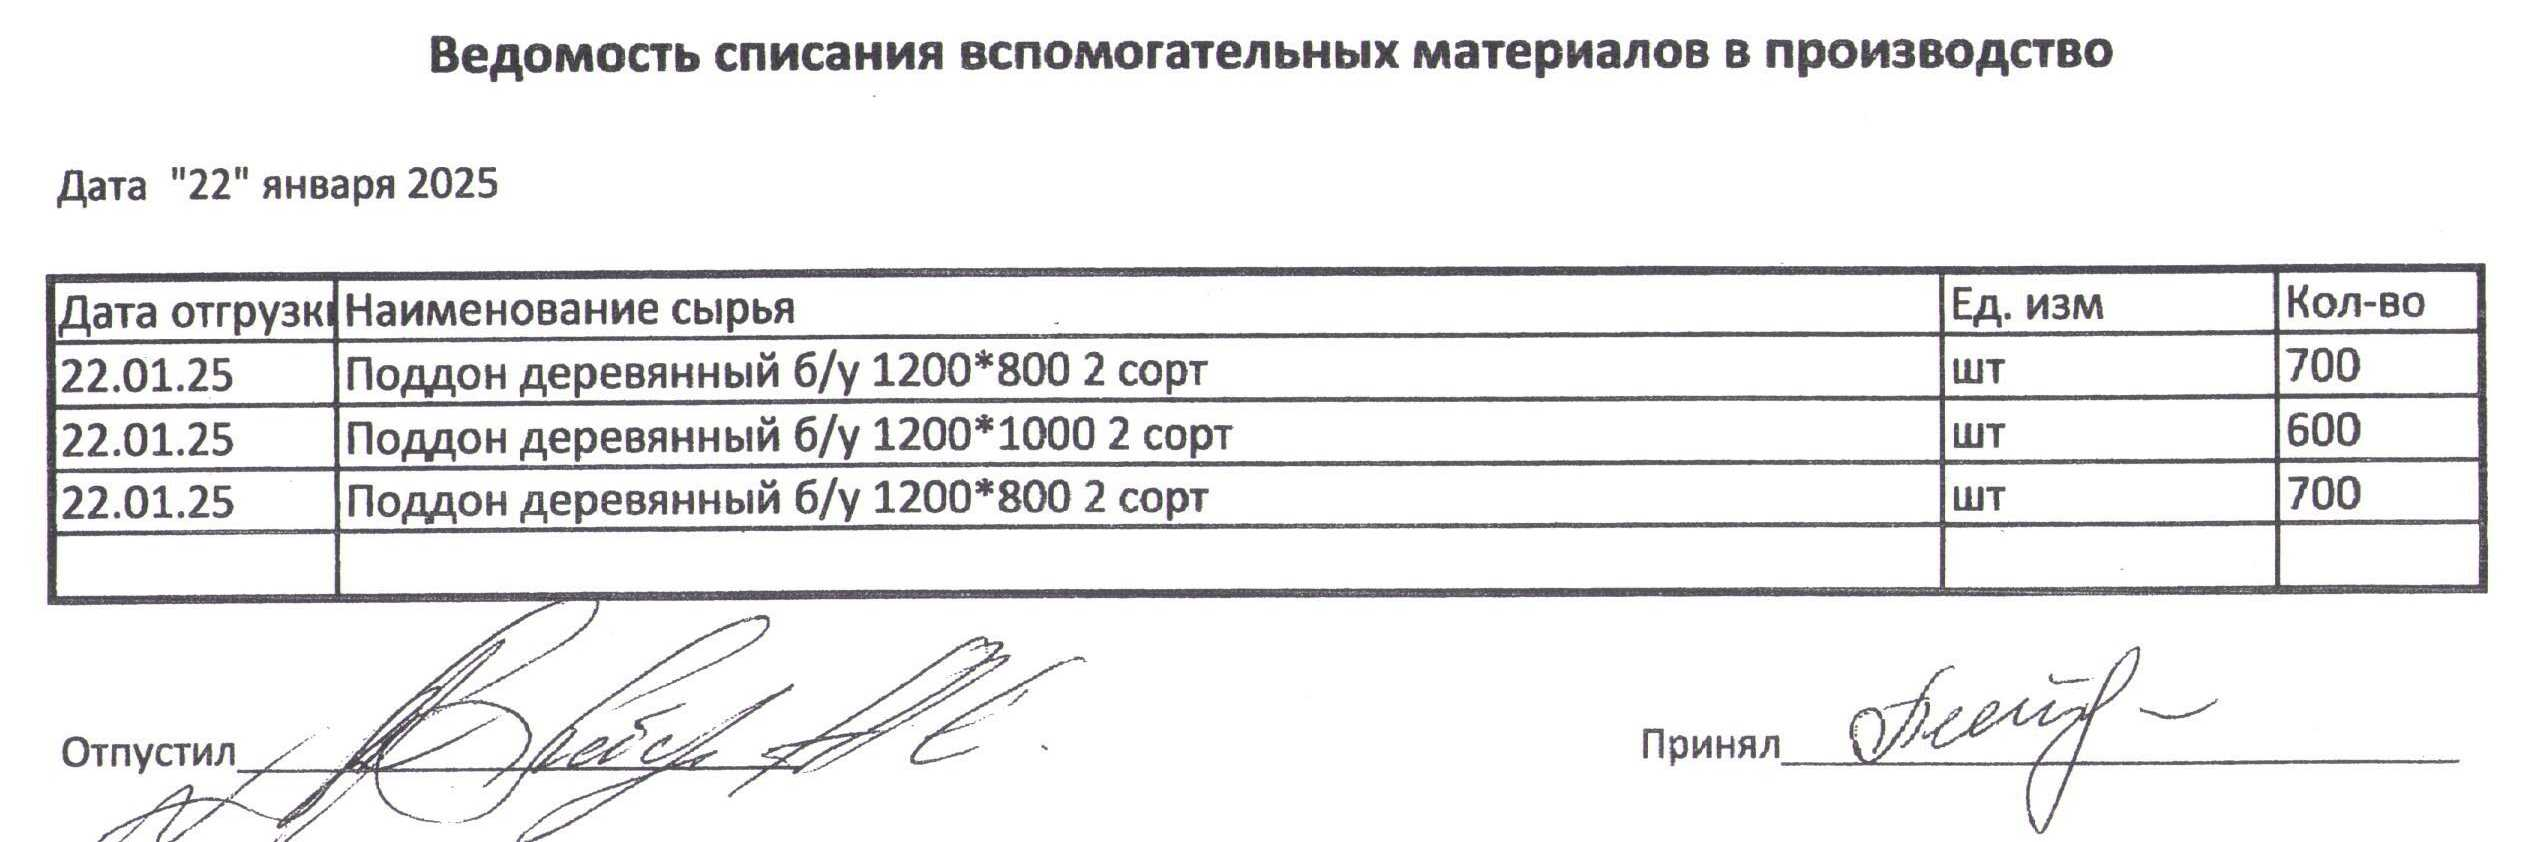
\includegraphics[height=0.94\textheight, width=\textwidth, keepaspectratio]{Pics/f27.jpg}
\end{center}
\caption{Ведомость списания вспомогательных материалов в производство}
\label{pic:f27}
\end{figure}

\clearpage
\ifx \notincludehead\undefined
\normalsize
\end{document}
\fi